% !TEX program = xelatex
% 目标导向多模态情感分类的复现实证研究（RethinkingTMSC 独立分析）
\documentclass[11pt]{ctexart}
\usepackage[a4paper,top=2.6cm,bottom=2.6cm,left=2.8cm,right=2.8cm]{geometry}
\usepackage{booktabs}
\usepackage{graphicx}
\usepackage{amsmath,amssymb}
\usepackage{float}
\usepackage{caption}
\usepackage{xcolor}
\usepackage{tabularx}
\usepackage[colorlinks=true,linkcolor=black,citecolor=black,urlcolor=blue]{hyperref}
\usepackage{titlesec}
\newcommand{\sectionbreak}{\clearpage}

\captionsetup{font=small,labelfont=bf}
\graphicspath{{../analysis/figures/}}
\setlength{\parskip}{0.25em}
\emergencystretch=2em

\title{\bfseries 目标导向多模态情感分类的复现实证研究\\[0.5em]
  \large ——以 RethinkingTMSC（EMNLP 2023 Findings）为例的独立分析}
\author{简相彪\\[0.5em]}
\date{2026 年 8 月}

\begin{document}

\maketitle

\begin{abstract}

目标导向多模态情感分类（Target-oriented Multimodal Sentiment Classification，TMSC）要求模型结合文本与图像判断推文中指定目标实体的情感极性。RethinkingTMSC（Ye et al., 2023）在 Twitter15 与 Twitter17 上系统比较了文本/图像单模态与多种多模态融合架构，发现现有系统主要依赖文本模态，图像带来的增益十分有限。本文以该工作为对象，完成三方面工作：（1）代码级可运行性验证，确认数据读取、特征构造、单模态与多模态模型的前向/反向传播在无 GPU 环境下亦可跑通，并整理出面向 GPU 服务器的完整复现脚本包；（2）基于作者随仓库公开的 220 组实验结果（2 数据集 $\times$ 22 模型 $\times$ 5 种子）进行系统再分析，包括均值/方差、种子稳定性、5 种子多数投票集成、相对文本基线的纠正/恶化统计、混淆矩阵与逐类指标；（3）对原始数据进行统计，并对全部模型都预测错误的困难样本进行挖掘。结果表明：纯视觉模型远弱于文本模型；多数多模态模型相对 BERT 的 F1 提升不足 1 个百分点甚至下降；种子随机性对部分模型（如 Faster2Bert）影响极大（准确率跨度最高达 17.7 个百分点）；5 种子投票集成能在绝大多数模型上带来稳定增益（最高 $+7.7$/$+17.7$ 个 F1 百分点）；负面情感与隐含/反讽表达是当前方法最主要的错误来源。上述发现为 TMSC 任务的数据建设、模型设计与评测协议提供了可操作的参考。
\end{abstract}

\noindent\textbf{关键词：}多模态情感分类；目标导向；复现研究；BERT；视觉编码器；种子稳定性


\section{引言}

社交媒体中的一条推文往往同时包含文字与配图，而用户对推文中某个具体实体（如某位明星、某支球队）的情感态度，可能与整条推文的情感并不一致。为此，Yu 和 Jiang（2019）提出目标导向多模态情感分类（TMSC）任务：给定文本、图像以及文本中的目标实体，判断该实体被表达的情感极性（负面/中性/正面），并构建了 Twitter15 与 Twitter17 两个英文数据集。此后，大量工作围绕视觉编码器与跨模态融合模块展开，方法日趋复杂，但两个数据集上的 F1 长期停留在 70\% 左右，进步缓慢。

RethinkingTMSC（Ye et al., 2023）对这一现象进行了实证剖析。作者固定文本编码器为 BERT（Devlin et al., 2019），分别采用 ResNet-152（He et al., 2016）、ViT-base（Dosovitskiy et al., 2021）与 Faster R-CNN（Ren et al., 2015）作为视觉编码器，在每种编码器下构建单模态基线以及多种融合变体，共 22 个模型 $\times$ 5 个随机种子，在两个数据集上进行统一评测。其核心结论是：图像模态的信息增益有限，多数目标的情感仅凭文本即可判定，因此简单而稳定的文本模型已经具有很强的竞争力。

本文并不是对原文的翻译，而是一次“复现 + 再分析”的独立实证研究，贡献如下：
\begin{enumerate}
  \item \textbf{复现工程}：逐行核查官方代码，完成 CPU 环境下的代码级冒烟验证，识别出若干影响复现的工程问题（硬编码路径、脚本工作目录、预训练权重路径、PyPI 依赖缺失等），并提供面向 GPU 服务器的一键复现脚本包（\texttt{repro/}）。
  \item \textbf{统计再分析}：对作者公开的 220 组结果重新聚合，给出均值$\pm$标准差、模型排序、种子方差；新增 5 种子多数投票集成分析，发现集成几乎总是带来正收益。
  \item \textbf{错误分析}：基于逐样本预测输出，计算混淆矩阵、逐类指标、相对文本基线的“纠正/恶化”样本数、按目标长度的错误率分层，并挖掘出全部 22 个模型均预测错误的困难样本，指出讽刺、反讽与隐含情感是主要失败模式。
  \item \textbf{数据观察}：给出两个数据集在标签分布、图片共享程度、目标长度等方面的量化统计，并结合模型表现讨论“图像何时有用”。
\end{enumerate}

\section{任务定义与基准方法}

\subsection{任务定义}

给定推文文本 $X=\{x_1,\ldots,x_n\}$、文本中指定的目标实体 $t$（在文本中以占位符 \texttt{\$T\$} 出现）以及配图 $I$，TMSC 的目标是预测标签 $y\in\{\text{负面},\text{中性},\text{正面}\}$。评测指标为准确率（Acc）与宏平均 F1（Macro-F1），与原文一致。

\subsection{模型体系}

官方代码将模型按视觉编码器分为三组，每组内包含单模态基线与多种融合结构：
\begin{itemize}
  \item \textbf{文本基线 BERT}：以 \texttt{bert-base-uncased} 为文本编码器，将句子与目标拼接为 \texttt{[CLS] 句子 [SEP] 目标 [SEP]} 的输入形式（即 Yu 和 Jiang, 2019 的 mBERT 设定），仅利用文本。
  \item \textbf{纯视觉模型}：ResNet-152（49 个区域 $\times$ 2048 维）、ViT-base（197 个 patch 向量）、Faster R-CNN（36 个区域 $\times$ 2048 维，Visual Genome 预训练）。
  \item \textbf{融合模型}：简单拼接类（ResBert / VitBert / FasterBert）、双线性张量融合 TFN（Zadeh et al., 2017）变体（ResBertTFN / VitBertTFN / FasterBertTFN）、MBERT 类（Res2Bert、Bert2Res、Res22Bert 及其 Vit/Faster 对应物）以及注意力类（ResBertAtt / VitBertAtt / FasterBertAtt）。
\end{itemize}

\subsection{统一训练与评测协议}

全部实验采用统一设置：8 个 epoch、batch size 32、学习率 $2\times10^{-5}$、5 个随机种子（0/42/199/2022/11122）；每轮在开发集上评测，按开发集准确率保存最优检查点，训练结束后加载最优检查点在测试集上评测；测试结果写入 \texttt{eval\_results.txt}。损失函数为广义交叉熵（GCELoss，$q=0$ 时退化为标准交叉熵），优化器为带线性 warmup 的 BertAdam。图像侧在特征构造阶段进行随机裁剪与水平翻转增强。

\section{数据集分析}\label{sec:data}

表~\ref{tab:data} 给出两个数据集的统计结果。Twitter15 的标签分布严重偏向中性（约 59\%），而 Twitter17 相对均衡。两个数据集中，每条推文的目标平均只有约 1.6 个词，文本平均约 16 个词。一个值得注意的差异是\textbf{图片共享程度}：Twitter15 全部 5338 个样本对应 3502 张去重图片（38\% 的图片被 2 个及以上样本共用），Twitter17 全部 5972 个样本对应 2908 张图片（66.5\% 的图片被 2 个及以上样本共用）。即 Twitter17 中“同图多目标、多情感”的情况更普遍，图片与目标之间的关系更复杂，也更考验模型对目标与图像内容的对齐能力。

\begin{table}[htbp]
\centering
\caption{Twitter15 / Twitter17 数据集统计}\label{tab:data}
\footnotesize
\resizebox{\textwidth}{!}{%
\begin{tabular}{lcccccccc}
\toprule
数据集 & 划分 & 样本数 & 负面(\%) & 中性(\%) & 正面(\%) & 去重图片 & 平均每图样本 & 目标平均词数 \\
\midrule
Twitter15 & train & 3179 & 11.6 & 59.2 & 29.2 & --- & --- & 1.66 \\
Twitter15 & dev   & 1122 & 13.3 & 59.7 & 27.0 & --- & --- & 1.68 \\
Twitter15 & test  & 1037 & 10.9 & 58.5 & 30.6 & --- & --- & 1.68 \\
Twitter15 & 全部  & 5338 & --- & --- & --- & 3502 & 1.52 & --- \\
Twitter17 & train & 3562 & 11.7 & 46.0 & 42.3 & --- & --- & 1.65 \\
Twitter17 & dev   & 1176 & 12.2 & 44.0 & 43.8 & --- & --- & 1.62 \\
Twitter17 & test  & 1234 & 13.6 & 46.4 & 40.0 & --- & --- & 1.59 \\
Twitter17 & 全部  & 5972 & --- & --- & --- & 2908 & 2.05 & --- \\
\bottomrule
\end{tabular}}
\caption*{\footnotesize 注：多数类基线（全部预测中性）在 Twitter15 / Twitter17 测试集上的准确率分别为 58.53\% 与 46.43\%。文本平均约 16 词，未列入表中。}
\end{table}

\begin{figure}[htbp]
\centering
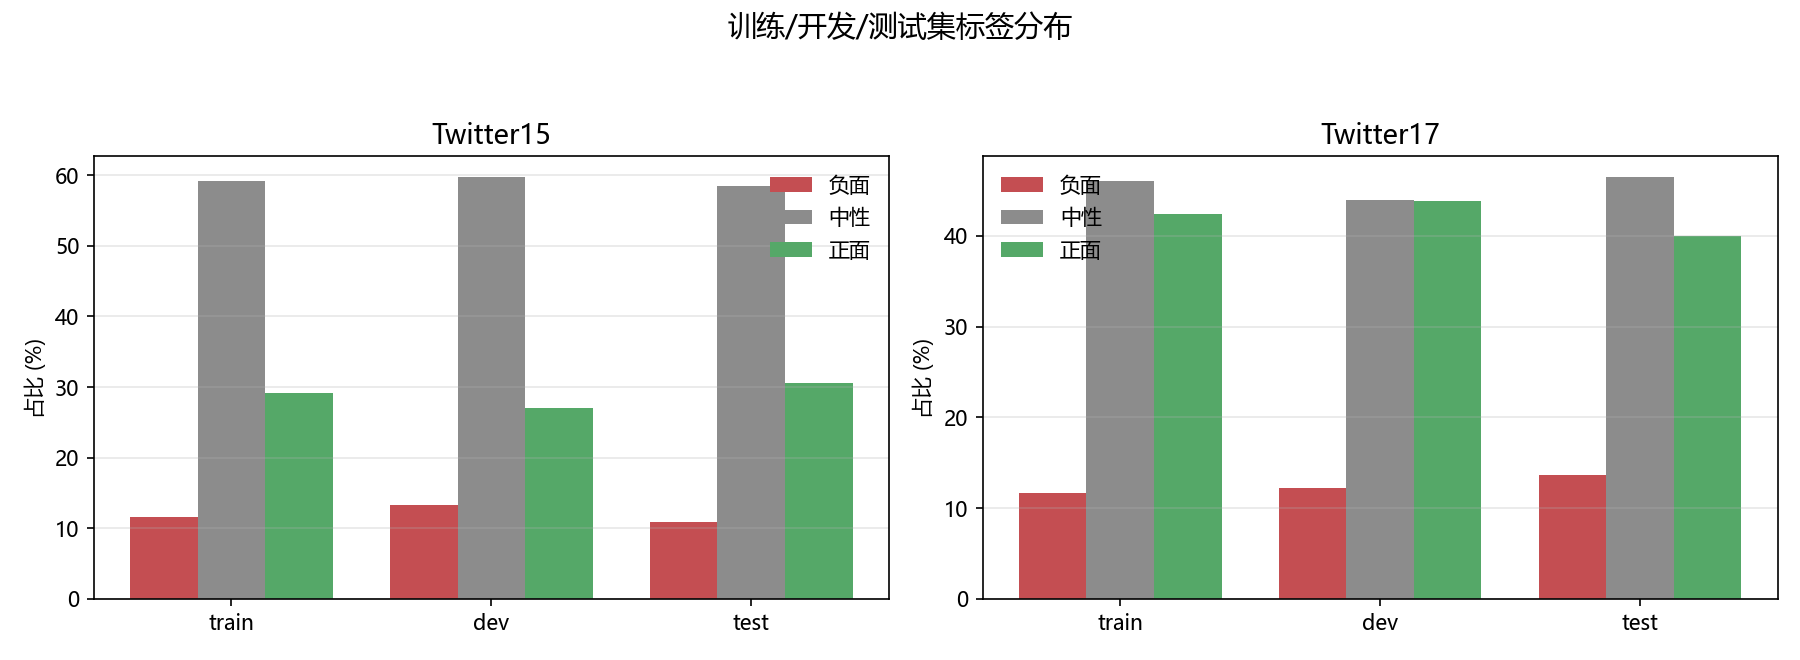
\includegraphics[width=0.92\textwidth]{fig5_label_dist.png}
\caption{两个数据集的标签分布（负面/中性/正面占比）}\label{fig:label}
\end{figure}

\section{复现设置与可行性}

\subsection{本机环境与限制}

本文的代码级验证在本机（Windows，CPU-only，torch 1.10.0+cpu，transformers 4.22.1）完成。经核查，完整训练复现需要的条件中：推文图片数据与预训练权重均已就绪（原始 IJCAI2019 数据集解压于 \texttt{data/twitter2015\_images/} 与 \texttt{data/twitter2017\_images/}，经核对与 tsv 的 ImageID 完全对应，Twitter15 3502 张、Twitter17 2908 张、缺失 0 张，并已整理到官方要求的 \texttt{data/<数据集>/images/}；ResNet-152 权重位于 \texttt{Code/resnet/resnet152.pth}，Faster R-CNN 权重位于 \texttt{Code/faster\_rcnn/models/}\allowbreak\texttt{faster\_rcnn\_res101\_vg.pth}）。本机仍不具备的条件是：（1）NVIDIA GPU（22 模型 $\times$ 2 数据集 $\times$ 5 种子共 220 次 BERT 级微调，CPU 上不现实）；（2）BERT/ViT 权重需首次运行时联网从 Hugging Face 下载（本机缓存为空、网络受限）。

因此，本文采取“代码冒烟验证 + 作者公开结果再分析 + 服务器复现包”三管齐下的策略：（1）在 CPU 上验证官方代码链路可运行；（2）对作者随仓库公开的 220 组测试结果（\texttt{output/}，即论文报告结果）做独立的统计与错误分析；（3）提供 \texttt{repro/} 一键脚本包，供在租用 GPU 服务器上完成真正的训练复现，复现完成后可将结果与本文表格对照。

\subsection{代码级冒烟验证}\label{sec:smoke}

为了确认官方代码并非“纸面可运行”，我们编写了 \texttt{analysis/smoke\_test.py}：在无预训练权重、无 GPU 的条件下，用随机图像张量与随机初始化的微型 BERT（2 层、hidden=64）走通完整链路，并额外用真实推文图片验证图片加载路径，结果如下：
\begin{itemize}
  \item Tsv 读取与 \texttt{AbmsaProcessor} 数据解析正常，8 条开发集样本全部成功构造 \texttt{MMInputFeatures}（含目标序列与 $3\times224\times224$ 图像特征）；
  \item BERT 前向/反向 + BertAdam 两步训练正常（loss $\approx 1.10$），梯度正常传播；
  \item BERT 推理输出形状 (batch, 3) 正确；
  \item 多模态模型 \texttt{Res22Bert}（文本-图像交叉注意力）前向/反向正常（loss $\approx 1.06$）；
  \item 真实推文图片经 ResNet 路径的随机裁剪、归一化后输出形状正确（$3\times224\times224$）。
\end{itemize}

上述结果说明官方代码的主链路（数据 $\rightarrow$ 特征 $\rightarrow$ 训练 $\rightarrow$ 推理 $\rightarrow$ 图片加载）可以执行；真正影响完整复现的只是算力与预训练权重等外部资源，而非代码本身。

\subsection{结果口径说明}

第~\ref{sec:results}~节的定量结果基于作者随仓库公开的 \texttt{output/}（论文报告结果）：每个模型在每个数据集上有 5 个种子的 \texttt{eval\_results.txt}。我们以均值$\pm$标准差呈现，并新增了原文未报告的投票集成、纠正/恶化与分层错误率分析。待服务器复现完成后，可将 \texttt{repro/collect\_results.py} 生成的 \texttt{results\_summary.csv} 与本文表~\ref{tab:t15}、表~\ref{tab:t17} 直接对比。

\section{结果与实证分析}\label{sec:results}

\subsection{全模型结果}

表~\ref{tab:t15} 与表~\ref{tab:t17} 分别给出两个数据集上 22 个模型的 5 种子均值$\pm$标准差，图~\ref{fig:f1} 为可视化。所有数值均为百分比。

\begin{table}[htbp]
\centering
\caption{Twitter15 测试集结果（5 种子均值$\pm$标准差，\%）}\label{tab:t15}
\footnotesize
\resizebox{\textwidth}{!}{%
\begin{tabular}{lcccc}
\toprule
模型 & 视觉编码器 & Acc & Macro-F1 & 最佳种子 F1 \\
\midrule
Bert & --- & 76.72 $\pm$ 1.29 & 71.19 $\pm$ 2.45 & 73.30 \\
ResNet & ResNet-152 & 57.65 $\pm$ 1.11 & 32.52 $\pm$ 2.97 & 35.51 \\
Vit & ViT-base & 59.65 $\pm$ 1.27 & 31.25 $\pm$ 3.04 & 34.03 \\
FasterRCNN & Faster R-CNN & 55.97 $\pm$ 1.22 & 35.72 $\pm$ 6.07 & 42.45 \\
ResBert & ResNet-152 & 75.29 $\pm$ 0.50 & 68.71 $\pm$ 1.50 & 70.41 \\
ResBertTFN & ResNet-152 & 74.19 $\pm$ 1.05 & 68.92 $\pm$ 0.64 & 69.71 \\
Res2Bert & ResNet-152 & 75.18 $\pm$ 1.85 & 67.77 $\pm$ 5.38 & 70.31 \\
Bert2Res & ResNet-152 & 77.13 $\pm$ 1.49 & 71.48 $\pm$ 2.12 & 74.79 \\
\textbf{Res22Bert} & ResNet-152 & \textbf{77.32 $\pm$ 0.70} & \textbf{72.06 $\pm$ 0.90} & 72.73 \\
ResBertAtt & ResNet-152 & 76.03 $\pm$ 1.08 & 70.57 $\pm$ 2.67 & 72.89 \\
VitBert & ViT-base & 76.22 $\pm$ 1.01 & 70.37 $\pm$ 1.62 & 72.77 \\
VitBertTFN & ViT-base & 73.44 $\pm$ 0.87 & 67.46 $\pm$ 1.62 & 69.38 \\
Vit2Bert & ViT-base & 75.12 $\pm$ 1.13 & 69.40 $\pm$ 1.55 & 71.28 \\
Bert2Vit & ViT-base & 77.11 $\pm$ 0.49 & 71.91 $\pm$ 0.47 & 72.18 \\
Vit22Bert & ViT-base & 76.70 $\pm$ 0.84 & 71.67 $\pm$ 1.62 & 73.56 \\
VitBertAtt & ViT-base & 75.08 $\pm$ 0.46 & 68.94 $\pm$ 0.93 & 69.89 \\
FasterBert & Faster R-CNN & 75.45 $\pm$ 0.82 & 69.78 $\pm$ 1.37 & 71.26 \\
FasterBertTFN & Faster R-CNN & 72.09 $\pm$ 0.74 & 66.77 $\pm$ 1.16 & 68.53 \\
Faster2Bert & Faster R-CNN & 70.82 $\pm$ 3.34 & 57.94 $\pm$ 6.50 & 65.13 \\
Bert2Faster & Faster R-CNN & 77.36 $\pm$ 0.42 & 71.69 $\pm$ 0.41 & 72.11 \\
Faster22Bert & Faster R-CNN & 76.57 $\pm$ 0.51 & 70.88 $\pm$ 0.99 & 72.06 \\
FasterBertAtt & Faster R-CNN & 76.08 $\pm$ 0.99 & 70.08 $\pm$ 1.53 & 71.34 \\
\bottomrule
\end{tabular}}
\end{table}

\begin{table}[htbp]
\centering
\caption{Twitter17 测试集结果（5 种子均值$\pm$标准差，\%）}\label{tab:t17}
\footnotesize
\resizebox{\textwidth}{!}{%
\begin{tabular}{lcccc}
\toprule
模型 & 视觉编码器 & Acc & Macro-F1 & 最佳种子 F1 \\
\midrule
Bert & --- & 68.04 $\pm$ 0.45 & 65.66 $\pm$ 0.39 & 66.10 \\
ResNet & ResNet-152 & 57.80 $\pm$ 1.11 & 51.98 $\pm$ 1.38 & 53.11 \\
Vit & ViT-base & 59.53 $\pm$ 1.07 & 54.08 $\pm$ 0.88 & 55.39 \\
FasterRCNN & Faster R-CNN & 56.18 $\pm$ 0.95 & 49.88 $\pm$ 1.91 & 52.50 \\
ResBert & ResNet-152 & 67.93 $\pm$ 0.62 & 65.32 $\pm$ 0.59 & 65.91 \\
ResBertTFN & ResNet-152 & 66.66 $\pm$ 1.35 & 63.99 $\pm$ 1.81 & 65.66 \\
Res2Bert & ResNet-152 & 68.07 $\pm$ 0.65 & 65.18 $\pm$ 1.65 & 66.24 \\
Bert2Res & ResNet-152 & 69.37 $\pm$ 0.41 & 66.85 $\pm$ 0.88 & 67.99 \\
Res22Bert & ResNet-152 & 68.41 $\pm$ 1.13 & 66.39 $\pm$ 1.55 & 68.19 \\
ResBertAtt & ResNet-152 & 68.01 $\pm$ 1.07 & 65.41 $\pm$ 1.78 & 66.95 \\
VitBert & ViT-base & 67.94 $\pm$ 0.79 & 66.17 $\pm$ 0.88 & 67.07 \\
VitBertTFN & ViT-base & 65.46 $\pm$ 1.86 & 62.02 $\pm$ 1.56 & 63.88 \\
Vit2Bert & ViT-base & 67.52 $\pm$ 1.19 & 64.49 $\pm$ 1.63 & 66.13 \\
Bert2Vit & ViT-base & 69.14 $\pm$ 0.58 & 66.96 $\pm$ 0.76 & 67.85 \\
Vit22Bert & ViT-base & 69.16 $\pm$ 0.19 & 67.25 $\pm$ 0.63 & 67.83 \\
VitBertAtt & ViT-base & 67.52 $\pm$ 0.65 & 65.55 $\pm$ 0.39 & 66.01 \\
FasterBert & Faster R-CNN & 67.60 $\pm$ 1.28 & 64.74 $\pm$ 1.90 & 67.23 \\
FasterBertTFN & Faster R-CNN & 66.34 $\pm$ 1.63 & 62.96 $\pm$ 2.34 & 64.81 \\
Faster2Bert & Faster R-CNN & 60.31 $\pm$ 7.18 & 54.51 $\pm$ 7.90 & 61.06 \\
Bert2Faster & Faster R-CNN & 68.43 $\pm$ 0.72 & 66.44 $\pm$ 1.23 & 68.39 \\
\textbf{Faster22Bert} & Faster R-CNN & \textbf{69.51 $\pm$ 0.69} & \textbf{67.50 $\pm$ 0.42} & 67.95 \\
FasterBertAtt & Faster R-CNN & 68.09 $\pm$ 1.23 & 66.12 $\pm$ 1.38 & 67.81 \\
\bottomrule
\end{tabular}}
\end{table}

\begin{figure}[htbp]
\centering
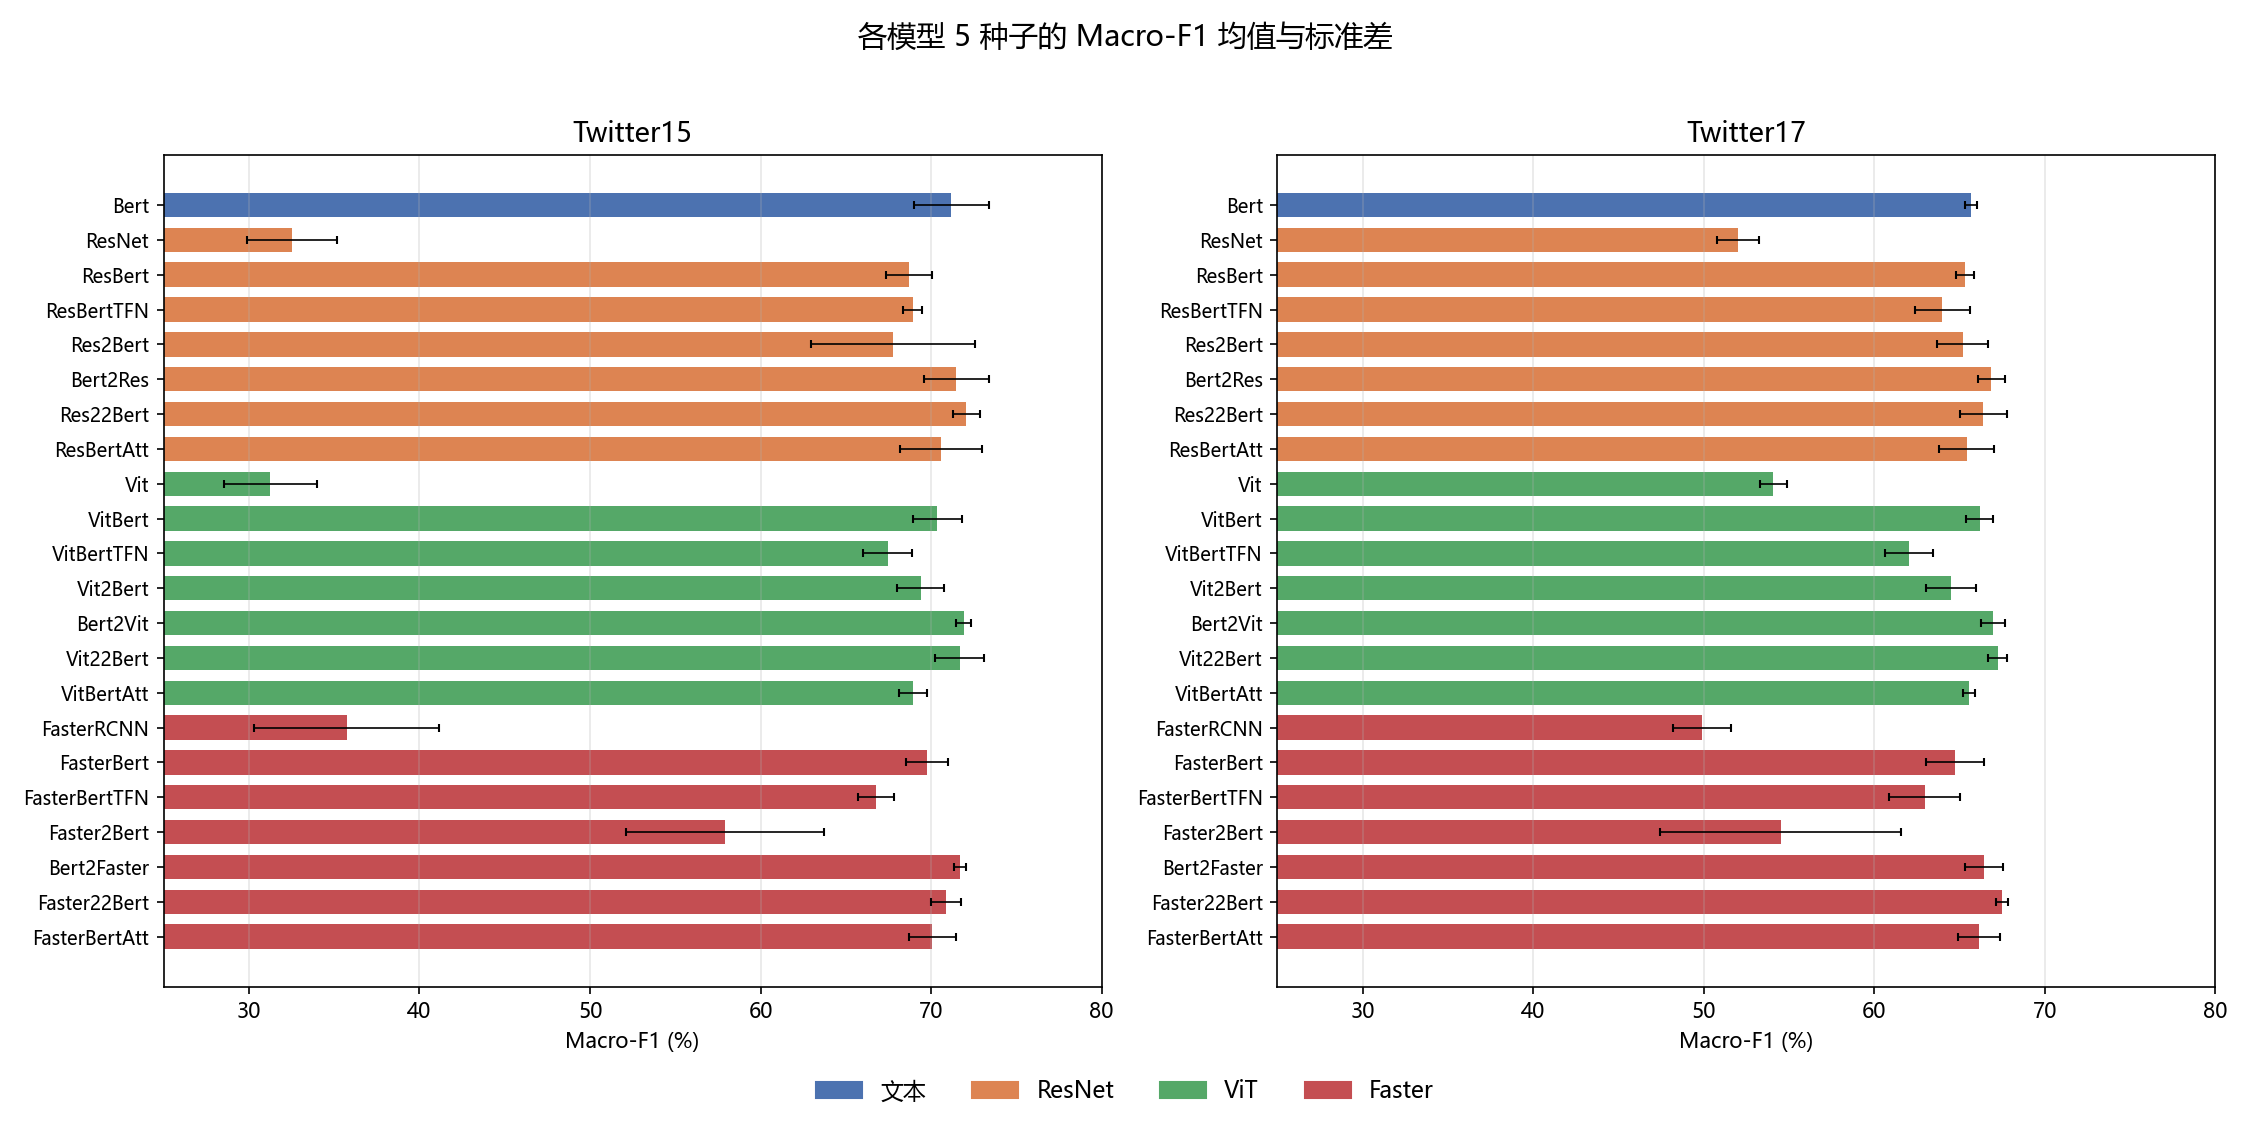
\includegraphics[width=0.95\textwidth]{fig1_f1_by_model.png}
\caption{两个数据集上各模型 Macro-F1 的均值与标准差（按视觉编码器着色）}\label{fig:f1}
\end{figure}

\subsection{单模态 vs 多模态：图像增益有限且不稳定}

三个纯视觉模型（ResNet / ViT / Faster R-CNN）在两个数据集上的 Macro-F1 仅为 31.3--54.1\%，远低于文本基线 BERT（65.7--71.2\%），与原文“模型主要依赖文本”的结论一致。

再看多模态融合模型相对 BERT 的差距：
\begin{itemize}
  \item \textbf{Twitter15}：21 个融合模型中有 16 个的 F1 均值低于 BERT；仅 Res22Bert（$+0.87$）、Bert2Vit（$+0.72$）、Bert2Faster（$+0.50$）、Vit22Bert（$+0.48$）等 5 个模型取得微弱正增益，最高也不足 1 个 F1 百分点。
  \item \textbf{Twitter17}：21 个融合模型中有 13 个低于 BERT；Faster22Bert（$+1.84$）、Vit22Bert（$+1.59$）、Bert2Vit（$+1.31$）、Bert2Res（$+1.19$）等取得正增益，幅度同样有限。
\end{itemize}

值得注意的是，\textbf{Twitter17 上的正增益模型数量更多、幅度更大}。结合第~\ref{sec:data}~节的数据观察，Twitter17 的图片共享程度更高、标签分布更均衡，图像内容与目标情感的相关性更强，这为“图像何时有用”提供了一个数据层面的解释：当图像与目标/情感的关系更紧密时，多模态融合才能带来可观测的收益。

\subsection{种子稳定性：部分模型“一次跑定生死”}

按模型计算 5 个种子准确率的极差（max$-$min）：
\begin{itemize}
  \item Twitter15 上，Faster2Bert 极差 8.4 个百分点（65.09--73.48），Res2Bert 4.5，其余模型大多在 1--3 个百分点之间；
  \item Twitter17 上，Faster2Bert 极差高达 \textbf{17.7 个百分点}（48.38--66.05），FasterBertTFN / VitBertTFN 等 TFN 类模型也超过 4 个百分点；
  \item 从标准差看，Twitter15 的 Res2Bert、Faster2Bert 的 F1 标准差分别达 5.4 与 6.5 个百分点，远高于同组其他模型。
\end{itemize}

这说明：（1）在 22 个模型中，个别模型（尤其 Faster2Bert 与部分 TFN 变体）的训练\textbf{极不稳定}，单次运行的结果不足以代表模型真实水平；（2）论文若只报告“最佳种子”或单次结果，可能会高估/低估某些方法；（3）评测协议应报告多次种子的均值$\pm$标准差，这也是本文建议后续研究采用的报告方式。

\subsection{新增分析：5 种子多数投票集成几乎总是“稳赚”}

原文未报告多种子集成。本文利用作者公开的 5 组预测做多数投票，得到以下发现（图~\ref{fig:ensemble}、表~\ref{tab:vote}）：
\begin{itemize}
  \item Twitter15：22 个模型中 20 个的投票 F1 $\geq$ 单种子（seed=0）F1；增益最大的三个模型为 ResBertAtt（$+7.71$）、VitBertTFN（$+5.66$）、Vit22Bert（$+5.19$），单位均为 F1 百分点；明显回退的只有本身就不稳定的 Faster2Bert（$-5.25$）与纯视觉 FasterRCNN（$-8.04$）。
  \item Twitter17：21/22 个模型投票不劣于单种子；Faster2Bert 因种子极不稳定，从投票中获益最多（$+16.32$）；投票后 Twitter17 的最佳模型为 Bert2Res（F1=68.71\%），超过任何单种子结果。
  \item 集成后 BERT 本身也从 66.02/73.19 提升到 66.76/73.37（Twitter17/Twitter15），说明\textbf{多数错误来自随机性而非系统性偏差}，简单集成即可稳定获得收益。
\end{itemize}

\begin{table}[htbp]
\centering
\caption{重点模型：单种子 vs 5 种子投票集成（Macro-F1，\%）}\label{tab:vote}
\footnotesize
\begin{tabular}{lcccc}
\toprule
数据集 & 模型 & seed=0 & 投票集成 & 差值 \\
\midrule
Twitter15 & Bert & 73.19 & 73.37 & $+0.18$ \\
Twitter15 & Vit22Bert & 69.20 & 74.39 & $+5.19$ \\
Twitter15 & ResBertAtt & 66.10 & 73.81 & $+7.71$ \\
Twitter15 & Faster2Bert & 65.13 & 59.88 & $-5.25$ \\
Twitter17 & Bert & 66.02 & 66.76 & $+0.75$ \\
Twitter17 & Bert2Res & 65.84 & 68.71 & $+2.87$ \\
Twitter17 & Faster2Bert & 41.38 & 57.71 & $+16.32$ \\
\bottomrule
\end{tabular}
\end{table}

\begin{figure}[htbp]
\centering
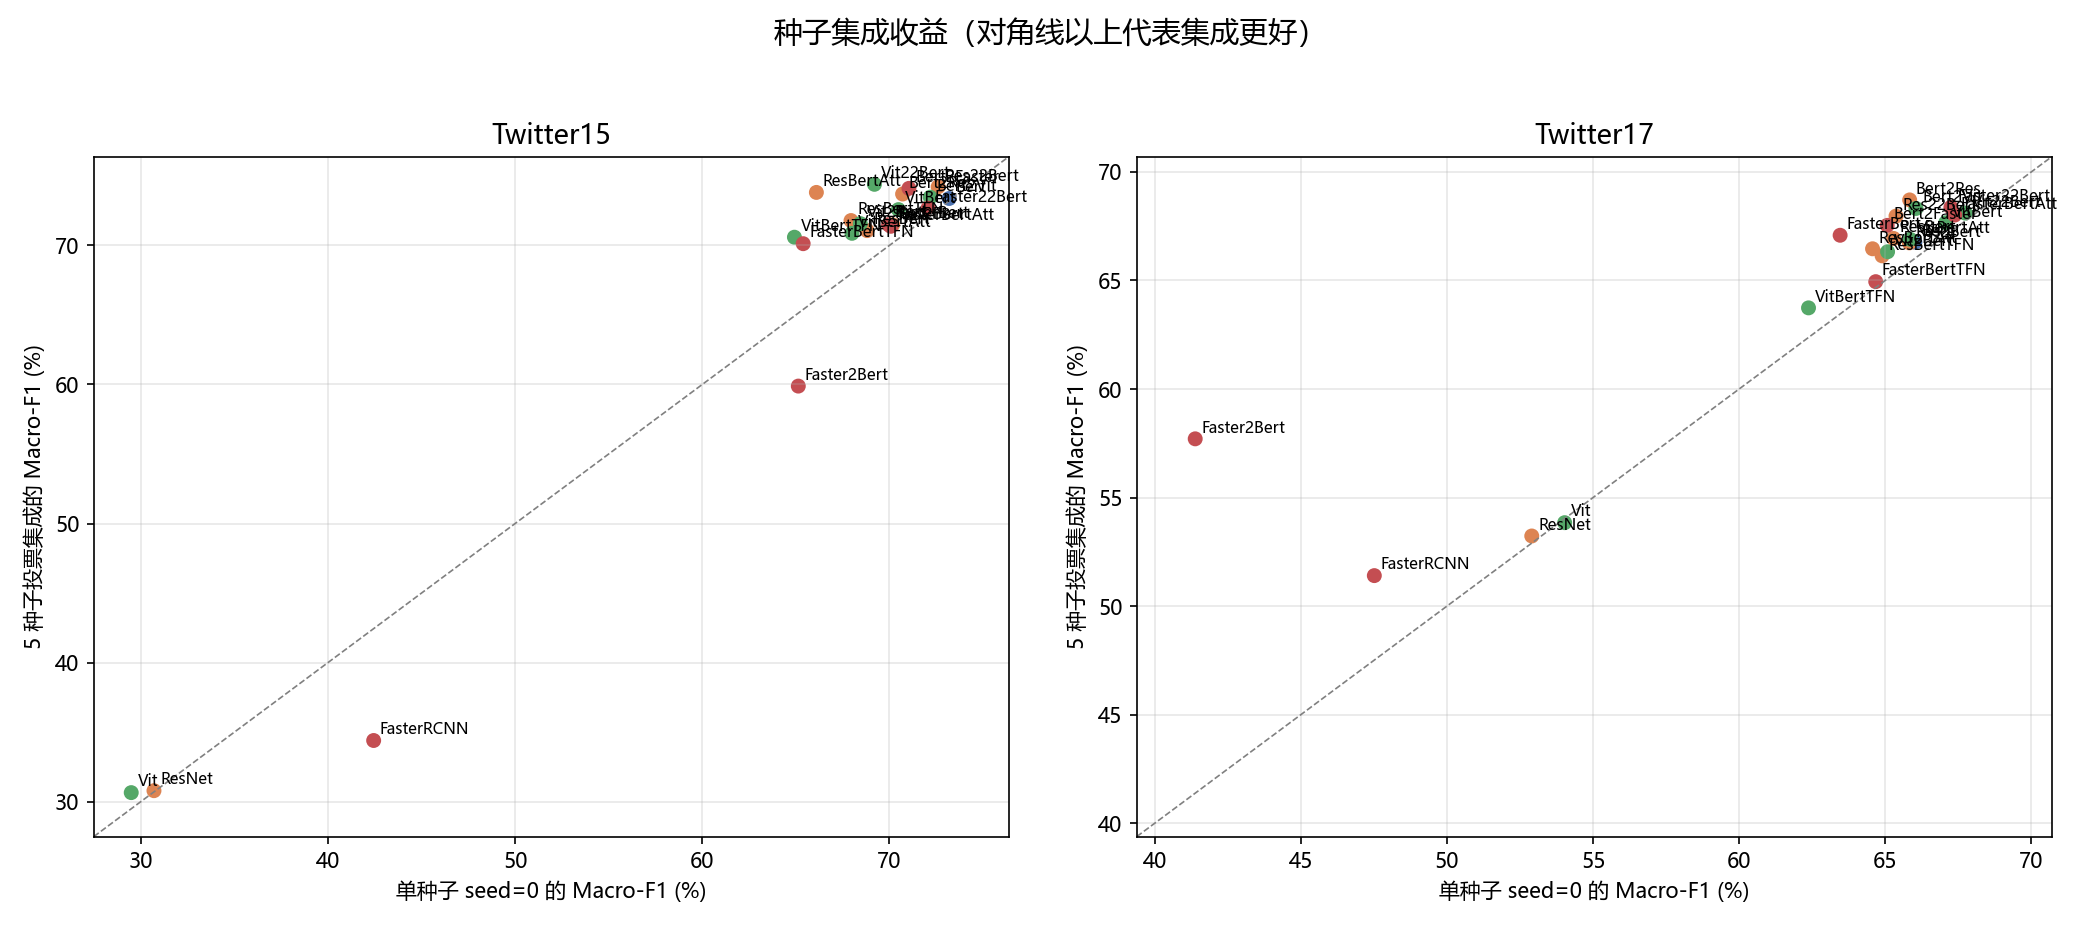
\includegraphics[width=0.88\textwidth]{fig4_ensemble.png}
\caption{5 种子投票集成与单种子（seed=0）的 Macro-F1 对比（对角线上方代表集成更好）}\label{fig:ensemble}
\end{figure}

\subsection{新增分析：多模态相对文本基线的“纠正/恶化”}

将每个多模态模型（seed=0）的预测与 BERT 逐样本比较，统计两类样本数：BERT 错而多模态对（纠正）、BERT 对而多模态错（恶化），结果见图~\ref{fig:corr}。

\begin{figure}[htbp]
\centering
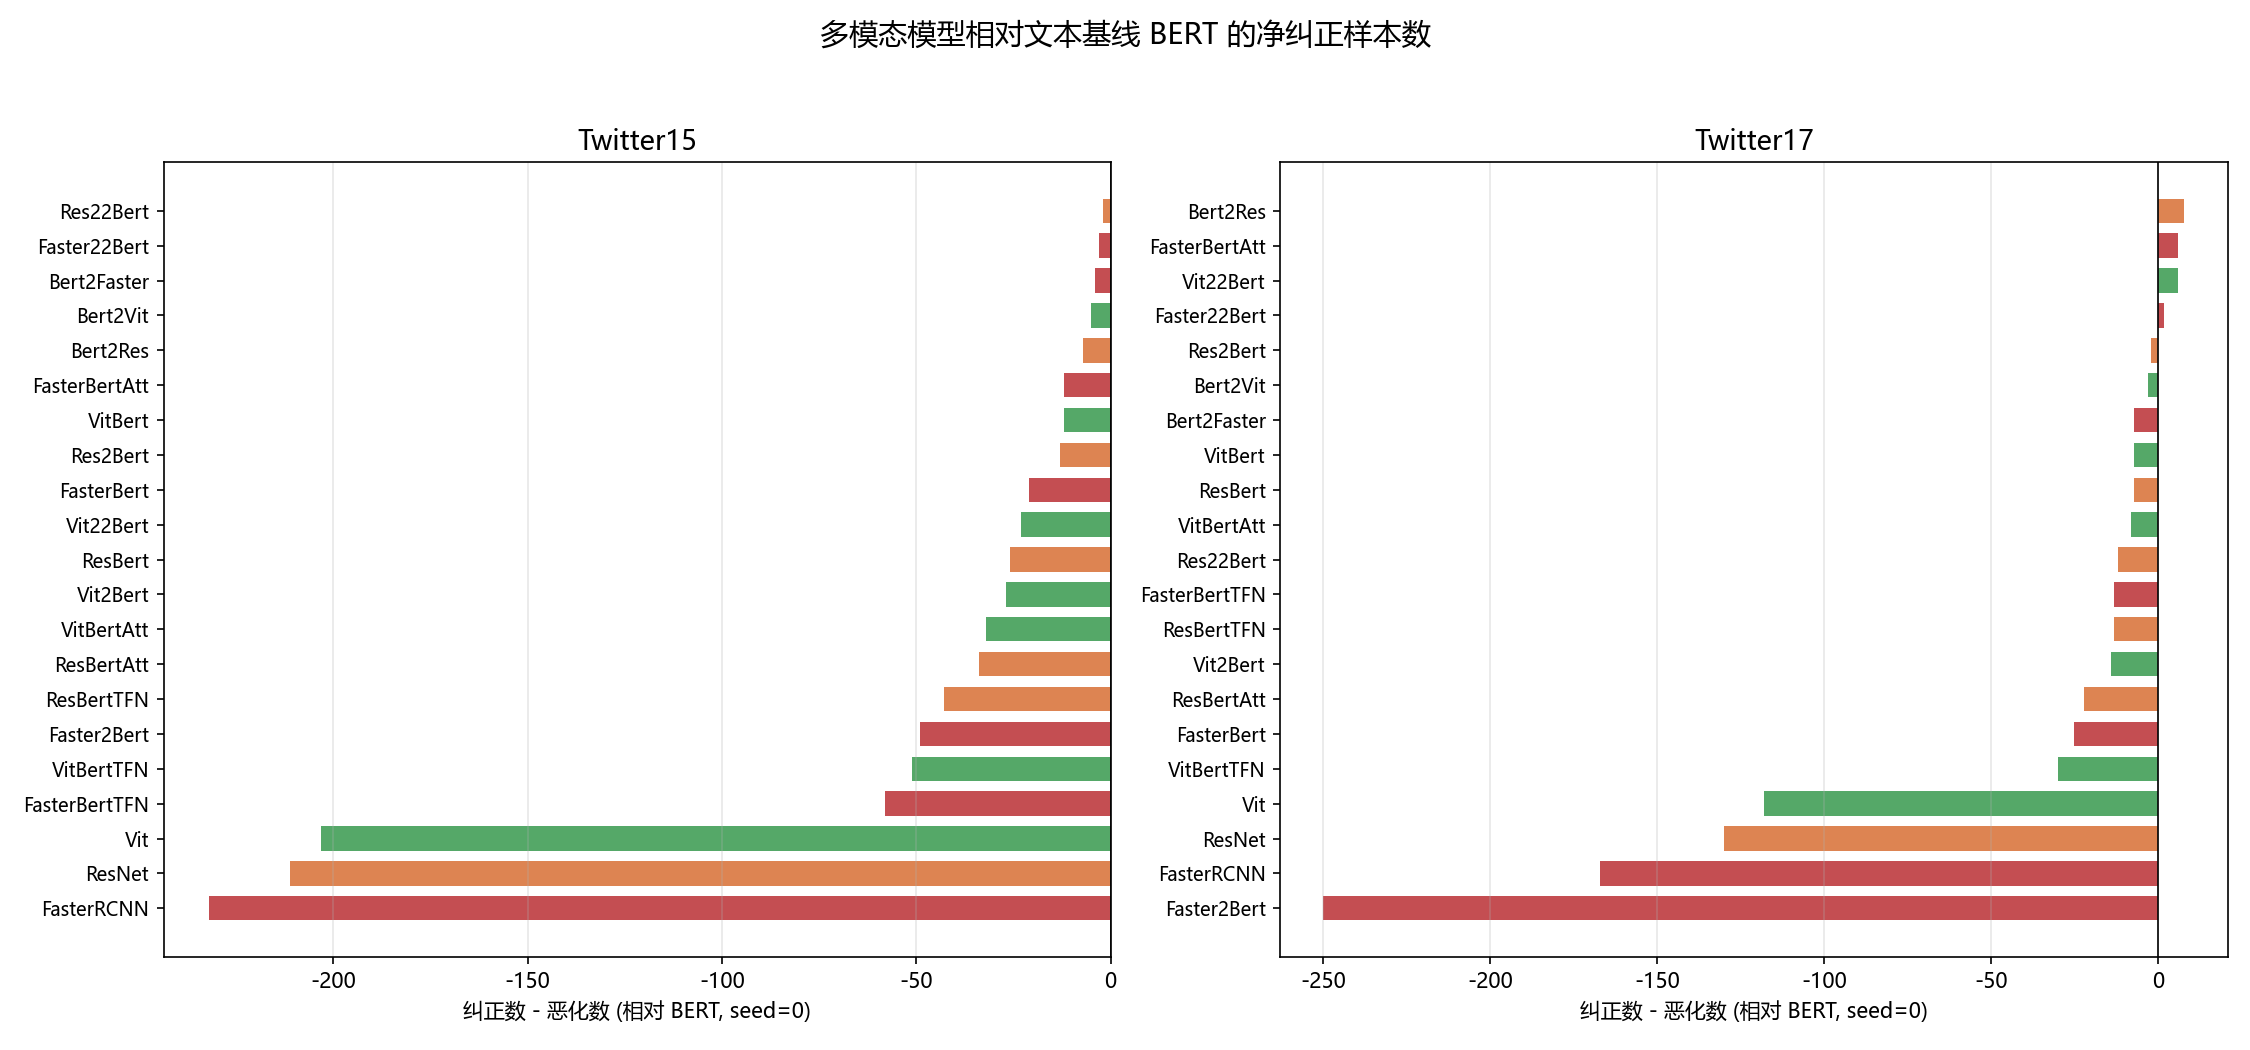
\includegraphics[width=0.95\textwidth]{fig3_correction_net.png}
\caption{多模态模型相对文本基线 BERT 的净纠正样本数（纠正$-$恶化，seed=0）}\label{fig:corr}
\end{figure}

\begin{itemize}
  \item \textbf{Twitter15}：21 个多模态模型全部净效应 $\leq 0$，即图像信息的引入总体上“弊大于利”：例如 Res22Bert 虽总 F1 略高于 BERT，但逐样本上仍为 $-2$（纠正 58 / 恶化 60）；TFN 类模型恶化明显（VitBertTFN $-51$、FasterBertTFN $-58$）。
  \item \textbf{Twitter17}：Bert2Res（$+8$）、FasterBertAtt（$+6$）、Vit22Bert（$+6$）、Faster22Bert（$+2$）等模型净效应为正，说明在图片与目标关联更强的 Twitter17 上，图像确实能“救回”一部分文本无法判定的样本；但多数模型仍为净负。
  \item 两个数据集上，BERT 与多模态模型的预测高度一致（逐模型统计：Twitter15 上约 69--72\% 的样本两者同时正确、约 16--17\% 同时错误；Twitter17 上约 60--61\% 同时正确、约 23--24\% 同时错误），真正不同的样本仅占约 10\%，这也是为什么总体 F1 差距很小。
\end{itemize}

\subsection{混淆矩阵与逐类指标}

图~\ref{fig:cm15} 与图~\ref{fig:cm17} 给出文本基线 BERT 与各数据集最优多模态模型（Twitter15 的 Res22Bert、Twitter17 的 Bert2Res）在 seed=0 下的混淆矩阵。两类模型均呈现相同模式：
\begin{itemize}
  \item Twitter15 上：中性类最易（F1=82.3），正面类次之（72.7），负面类最难（64.6）；
  \item Twitter17 上：正面类最易（F1=71.1），中性类次之（69.2），负面类最难（57.7）；
  \item 负面类在两个数据集上始终最难，因为负面情感常以反讽、隐晦方式表达；
  \item 错误主要发生在“负面 $\leftrightarrow$ 中性”与“正面 $\leftrightarrow$ 中性”之间，极少出现“负面 $\leftrightarrow$ 正面”的极性反转。
\end{itemize}

纯视觉模型则出现\textbf{类别坍缩}：ResNet / ViT / Faster R-CNN 几乎不预测负面类（负面类召回率极低甚至为 0），这也是其 F1 极低的原因——视觉模型在该任务上无法独立建模负面情感。

\begin{figure}[htbp]
\centering
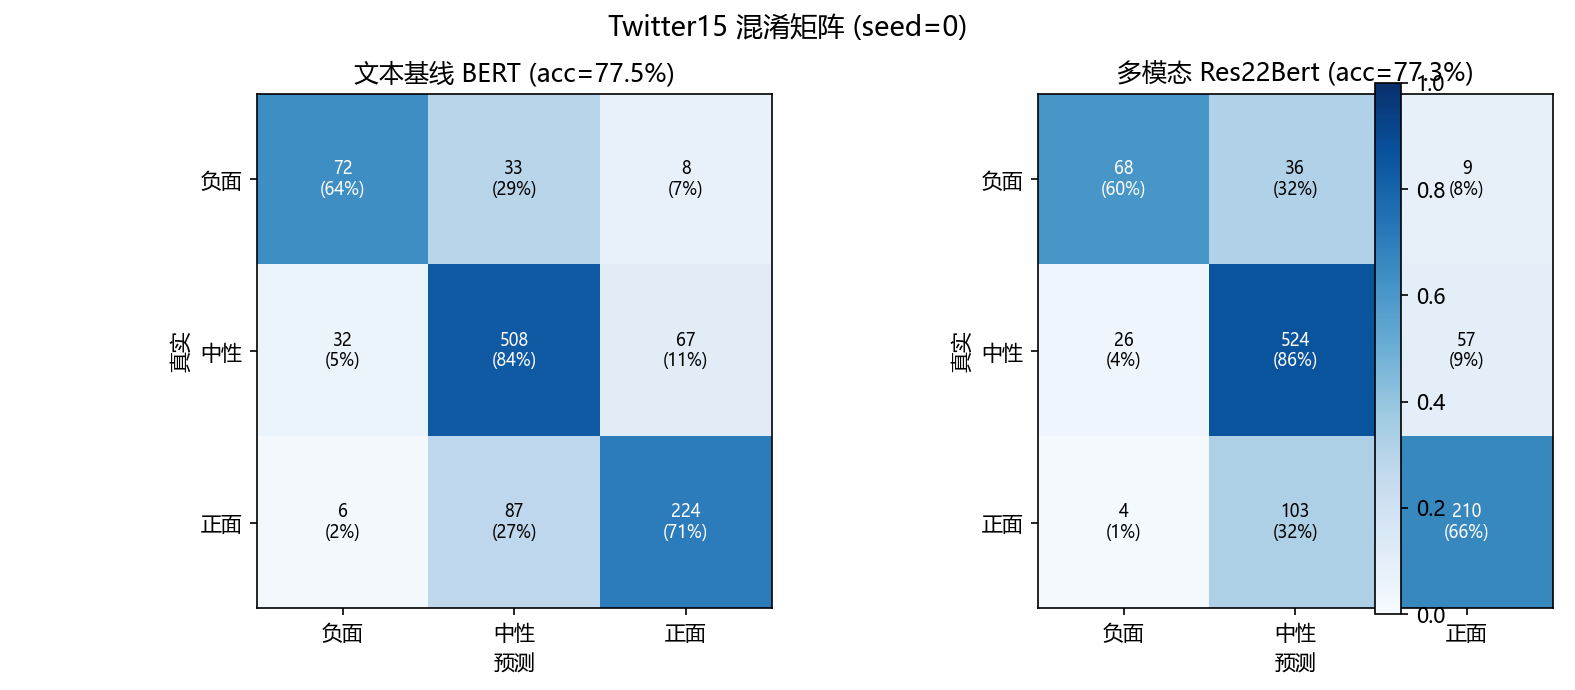
\includegraphics[width=0.78\textwidth]{fig2_confusion_Twitter15.png}
\caption{Twitter15：文本基线 BERT 与最优多模态模型（Res22Bert）的混淆矩阵（seed=0，行归一化）}\label{fig:cm15}
\end{figure}

\begin{figure}[htbp]
\centering
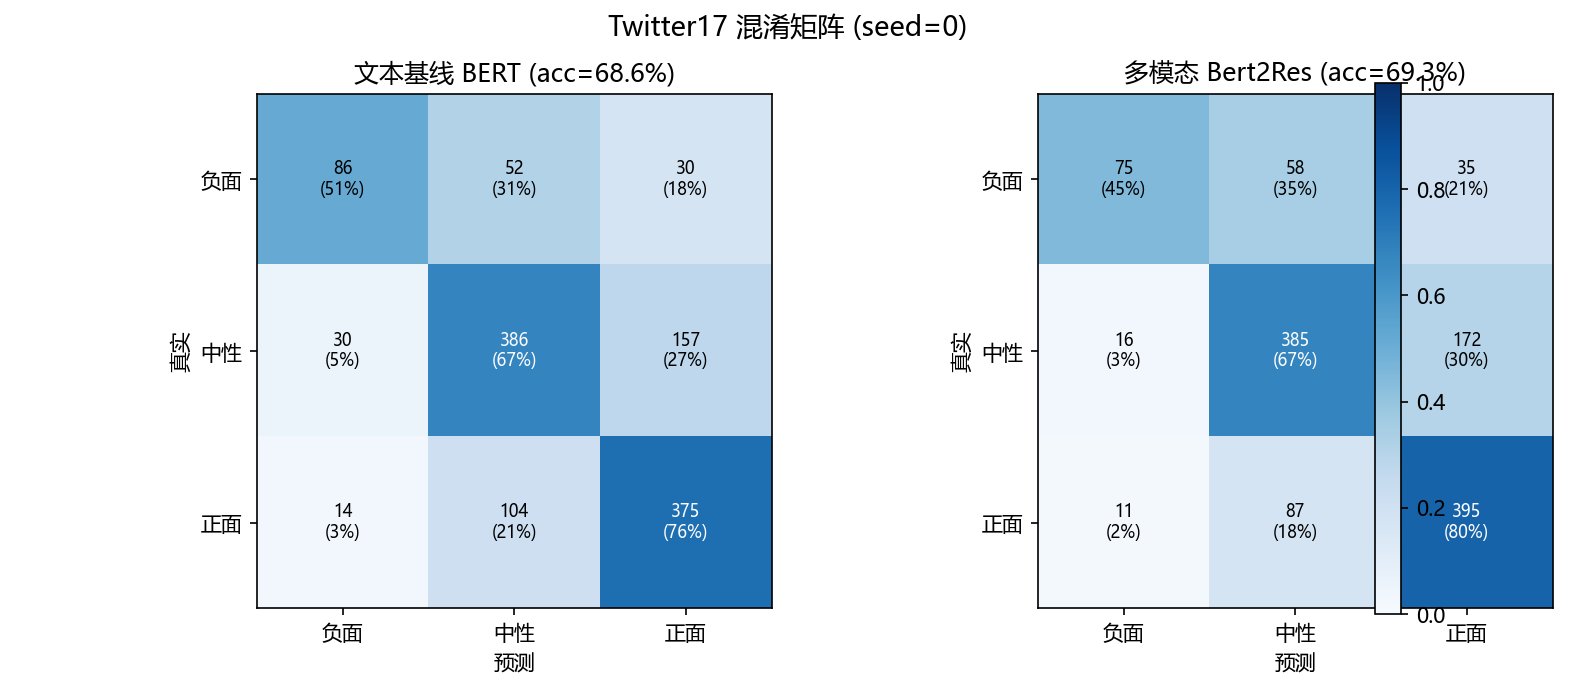
\includegraphics[width=0.78\textwidth]{fig2_confusion_Twitter17.png}
\caption{Twitter17：文本基线 BERT 与最优多模态模型（Bert2Res）的混淆矩阵（seed=0，行归一化）}\label{fig:cm17}
\end{figure}

\subsection{错误分层与困难样本}

按目标词数对 BERT（seed=0）的错误率分层（表~\ref{tab:errlen}）：

\begin{table}[htbp]
\centering
\caption{按目标词数的错误率（BERT, seed=0）}\label{tab:errlen}
\footnotesize
\begin{tabular}{lccc}
\toprule
数据集 & 目标 1 词 & 目标 2 词 & 目标 3+ 词 \\
\midrule
Twitter15 & 24.1\% & 21.7\% & 18.3\% \\
Twitter17 & 29.1\% & 33.4\% & 35.8\% \\
\bottomrule
\end{tabular}
\end{table}

两个数据集上目标长度与错误率的关系方向相反：Twitter15 上目标越长错误越少，Twitter17 上目标越长错误越多。一种可能的解释是：Twitter17 的长目标多为球队/联盟等集体实体（如 Premier League），其情感更依赖外部知识与上下文；而 Twitter15 的长目标常为专有名词，拼写特征本身即可提供较强的判别信号。该假设有待更大规模验证。

进一步，我们统计了每个测试样本被多少个模型（22 个模型 $\times$ seed=0）预测错误，挖掘出\textbf{全部 22 个模型都预测错误}的样本（表~\ref{tab:hard}）。这些样本几乎都是需要反讽理解或隐含常识的推文。

\begin{table}[htbp]
\centering
\caption{全部 22 个模型均预测错误的代表性样本}\label{tab:hard}
\footnotesize
\resizebox{\textwidth}{!}{%
\begin{tabular}{lclp{6.2cm}}
\toprule
数据集 & 真实标签 & 推文（节选） & 失败原因分析 \\
\midrule
Twitter15 & 负面 & Meet the Michael Jackson impersonator who wants to heal \$T\$ & 反讽：表面“治愈”实为负面 \\
Twitter15 & 正面 & Views from \$T\$ . No filter & 隐含情感：需结合图片才知是赞美风景 \\
Twitter15 & 负面 & Coretta Scott King with Robert amp \$T\$ after husband's assassination & 背景常识缺失 \\
Twitter17 & 负面 & Meek Mill beats \$T\$ , Kendrick Lamar , Future to win Top Rap Album... & 目标区分：同一句中多个实体，仅被提名者情感为负 \\
Twitter17 & 中性 & Me , along with a couple of friends --- James Franco and \$T\$ --- on the set... & 中性陈述但易被误判为正面 \\
Twitter17 & 负面 & @ \$T\$ Congrats ! You have went full Harry Reid stupid ! & 反讽式祝贺 \\
\bottomrule
\end{tabular}}
\end{table}

这些样本说明：当前 TMSC 模型的瓶颈不在“看不见图片”，而在\textbf{语言层面的反讽、隐含情感与实体区分}。仅提升视觉编码器或融合模块难以解决这类问题，需要更强的语言理解、常识推理或专门的训练数据。

\subsection{数据层面的补充观察}

\begin{itemize}
  \item Twitter15 测试集中有 113 个负面样本（10.9\%），模型负面类 F1 约 64\%；Twitter17 负面样本 168 个（13.6\%），负面类 F1 约 58--62\%——负面样本少且难，是 F1 上不去的直接原因。
  \item 两个数据集的测试集标签分布与训练/开发集基本一致，未见明显分布漂移。
  \item 所有样本的文本均含 \texttt{\$T\$} 占位符，目标以第二序列形式输入，这保证了目标信息在文本侧不会缺失；但\textbf{目标在图像中是否出现并未被约束}（Yu 和 Jiang, 2019 的标注也指出部分目标不出现在图中），这是数据本身对“多模态”定义的一个局限。
\end{itemize}

\section{复现性讨论}

\subsection{官方代码的工程问题}

在逐行核查与冒烟验证中，我们发现以下影响复现的工程问题（详见 \texttt{repro/README.md}）：
\begin{enumerate}
  \item \textbf{硬编码路径}：\texttt{run\_data\_analysis.py} 中图片目录写死为 \texttt{/root/RethinkingTMSC/...}，不在该路径下运行必然失败；复现脚本已自动替换为仓库实际路径。
  \item \textbf{脚本工作目录}：README 的 \texttt{cd scripts \&\& bash run.sh} 与脚本内相对路径矛盾，应在仓库根目录执行 \texttt{bash scripts/run.sh}。
  \item \textbf{权重路径}：\texttt{--resnet\_root} 默认 \texttt{./resnet} 与 README 要求的 \texttt{Code/resnet/} 不一致，且代码固定读取文件名 \texttt{resnet152.pth}，需显式传参并正确命名。
  \item \textbf{依赖缺失}：requirements.txt 中的 \texttt{apex}、\texttt{modeling} 在 PyPI 上不存在；apex 有 fallback（本文冒烟验证即证明无 apex 可运行），已从依赖中移除。
  \item \textbf{Faster* 模型}：需 Faster R-CNN 预训练权重（位于 \texttt{Code/faster\_rcnn/models/}\allowbreak\texttt{faster\_rcnn\_res101\_vg.pth}）及 CUDA 扩展编译；若编译失败，可用 \texttt{MODELS} 过滤跳过。
  \item \textbf{图片归属}：官方未提供自动整理脚本；本仓库已用 \texttt{data/twitter2015\_images/}、\allowbreak\texttt{data/twitter2017\_images/} 的图片整理完毕并逐张核对，若使用其他来源需自行核对 ImageID。
\end{enumerate}

\subsection{服务器复现指南}

\texttt{repro/} 目录提供了完整的一键式复现包：
\begin{verbatim}
bash repro/download_assets.sh   # 下载图片、ResNet-152、Faster R-CNN 权重
bash repro/setup_env.sh         # 建环境、修路径、编译 faster_rcnn
bash repro/run_all.sh           # 220 次训练（多卡/断点续跑/模型过滤）
python repro/collect_results.py Code/output   # 汇总结果 CSV
\end{verbatim}

复现完成后，将结果与表~\ref{tab:t15}、表~\ref{tab:t17} 对照：同种子下 F1 偏差在 $\pm 1$ 个百分点内可视为复现成功。

\section{结论与展望}

本文对 RethinkingTMSC 进行了独立的复现实证研究，主要结论如下：
\begin{enumerate}
  \item 官方代码主链路可运行（冒烟验证通过）；完整训练复现仅受限于算力、图片数据与预训练权重等外部资源，\texttt{repro/} 脚本包已就绪。
  \item 文本单模态 BERT 已具备很强性能；纯视觉模型远弱于文本模型且存在类别坍缩；多模态融合相对 BERT 的增益普遍不足 1 个 F1 百分点，且部分模型为负增益。
  \item 种子随机性影响显著：Faster2Bert 的准确率跨种子极差最高达 17.7 个百分点，单次运行报告不可靠；5 种子多数投票集成在 41/44 个“模型$\times$数据集”组合上不劣于单种子，最高带来 $+16.3$ 个 F1 百分点的提升。
  \item 错误集中在负面情感与反讽/隐含表达上；Twitter17 上图像的正向作用更大，与数据层图片共享程度更高一致。
\end{enumerate}

展望方面，我们认为有三个方向值得推进：一是\textbf{数据审计与重建}，约束目标在图像中的可见性并扩充负面与反讽样本；二是\textbf{更强的目标-图像对齐}（如 CLIP 类跨模态表示、检测框级目标定位），而非仅依赖整体图像特征；三是\textbf{评测协议规范化}，统一报告多种子均值$\pm$标准差并鼓励公开逐样本预测，以便他人进行本文这类再分析。

\begin{thebibliography}{9}
\bibitem{ye2023} Ye J, Zhou J, Tian J, et al. RethinkingTMSC: An Empirical Study for Target-Oriented Multimodal Sentiment Classification[C]. Findings of ACL: EMNLP 2023: 270--277.
\bibitem{yu2019} Yu J, Jiang J. Adapting BERT for Target-Oriented Multimodal Sentiment Classification[C]. IJCAI 2019: 5408--5414.
\bibitem{devlin2019} Devlin J, Chang M W, Lee K, et al. BERT: Pre-training of Deep Bidirectional Transformers for Language Understanding[C]. NAACL-HLT 2019: 4171--4186.
\bibitem{he2016} He K, Zhang X, Ren S, et al. Deep Residual Learning for Image Recognition[C]. CVPR 2016: 770--778.
\bibitem{dosovitskiy2021} Dosovitskiy A, Beyer L, Kolesnikov A, et al. An Image is Worth 16$\times$16 Words: Transformers for Image Recognition at Scale[C]. ICLR 2021.
\bibitem{ren2015} Ren S, He K, Girshick R, et al. Faster R-CNN: Towards Real-Time Object Detection with Region Proposal Networks[C]. NeurIPS 2015.
\bibitem{zadeh2017} Zadeh A, Chen M, Poria S, et al. Tensor Fusion Network for Multimodal Sentiment Analysis[C]. EMNLP 2017: 1103--1114.
\bibitem{zhang2018} Zhang Q, Fu J, Liu X, et al. Adaptive Co-attention Network for Named Entity Recognition in Tweets[C]. AAAI 2018: 5674--5681.
\bibitem{lu2018} Lu D, Neves L, Carvalho V, et al. Visual Attention Model for Name Tagging in Multimodal Social Media[C]. ACL 2018: 1990--1999.
\end{thebibliography}

\appendix
\section{数据、脚本与复现方法}

本文全部结果可由仓库内脚本复现：
\begin{itemize}
  \item \texttt{analysis/collect\_results.py}：汇总 220 组 \texttt{eval\_results.txt}，生成 \texttt{results\_all.csv} 与 \texttt{results\_summary.csv}（表~\ref{tab:t15}、表~\ref{tab:t17} 数据来源）。
  \item \texttt{analysis/data\_stats.py}：数据集统计（表~\ref{tab:data}）。
  \item \texttt{analysis/error\_analysis.py}：逐类指标、投票集成、纠正/恶化、困难样本（表~\ref{tab:vote}--表~\ref{tab:hard}）。
  \item \texttt{analysis/make\_figures.py}：图~\ref{fig:label}--图~\ref{fig:cm17}。
  \item \texttt{analysis/smoke\_test.py}：CPU 冒烟验证（第~\ref{sec:smoke}~节）。
  \item \texttt{repro/}：GPU 服务器复现包（第~6.2~节）。
\end{itemize}

所有分析脚本使用仓库自带虚拟环境 \texttt{TMSC\_env}（Python 3.8 + torch 1.10.0+cpu + transformers 4.22.1）运行，不依赖外部下载。

\end{document}
